\documentclass[10pt,a4]{article}
\usepackage[english]{babel}
\usepackage[utf8x]{inputenc}
\usepackage{amsmath}
\usepackage{float}
\usepackage{graphicx}
\usepackage{pdfpages}
\usepackage[colorinlistoftodos]{todonotes}
\usepackage{hyperref}
\usepackage{geometry}
\geometry{top=3cm,left=2cm,right=2cm,bottom=3cm}
\usepackage[scaled]{helvet}
\usepackage[T1]{fontenc}
\renewcommand\familydefault{\sfdefault}


\author{Federico Bocchieri}
\date{\today}
\title{Memorisation and replay of infrared remotes \\ [0.3cm] \Large Memorizzazione e replay di telecomando a infrarossi}

\begin{document}
\maketitle
\tableofcontents

\section{Project data}

\begin{itemize}
\item Project supervisors: prof. Federico Terraneo, prof. Daniele Cattaneo

\item Team members:
\begin{center}
\begin{tabular}{lll}
Last and first name & Person code & Email address\\
\hline
Federico Bocchieri & 10662633 & federico.bocchieri@mail.polimi.it
\end{tabular}
\end{center}

\item Federico (me) is the sole member of the group; also coming from previous knowledge from other courses, I have researched topics such as
\begin{itemize}
\item IR transmission and reception
\item Software sampling of digital signals
\item Microcontroller devices (timers, GPIOs, interrupt controllers)
\item Microcontroller programming using memory-mapped I/O
\end{itemize}
and carried out tasks of
\begin{itemize}
\item Implementing the required classes to read IR data and send out IR data
\item Configuring required microcontroller devices as per device manual
\item Writing ISRs and registering them
\item Verifying correctness using tools such as logic analyzers
\item Informal testing of its behaviour
\end{itemize}

\item Link to repository hosting source code \href{https://github.com/blvckmvgicdotexe/AOS_ES_Project}{here}
\end{itemize}

\section{Project description}

This project implements a tool to sample and replay low-frequency digital signals via infrared  such as those used in consumer electronics like TV / AC remotes.
It runs on the Miosix RTOS (maintained by prof. Terraneo and prof. Cattaneo) on a STMicroelectronics STM32 Nucleo F401RE board paired with the PMDB16 shield / hat specifically manufactured for the Sensor Systems course taught at Politecnico di Milano by prof. Federica Villa.




\subsubsection{The problem at hand: infrared transmission and reception}
Infrared communication typically consists of stimulating a receiver using a infrared light source.\\
In order to reject background light, the light source is modulated with a carrier wave at (typically) 38KHz, for example generated using PWM; on the receiver side, the received signal is demodulated and turned back into a series of zeroes and ones which in turn encode a message using some protocol like IR NEC.

\begin{figure}[H]
    \centering
    \begin{minipage}{0.48\textwidth}
        \centering
        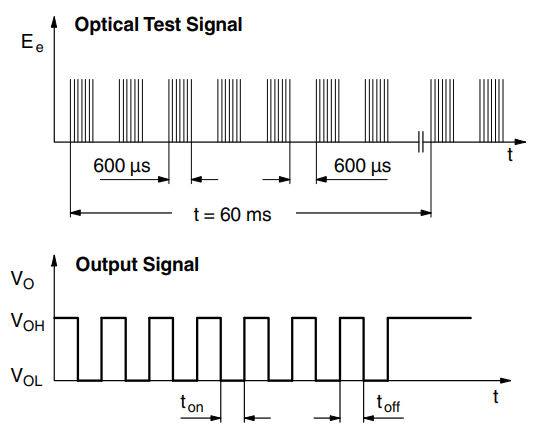
\includegraphics[width=\textwidth]{IR_demodulation.png}
        \caption{IR demodulation.}
        \label{fig:ir_demodulation}
    \end{minipage}
    \hfill
    \begin{minipage}{0.48\textwidth}
        \centering
        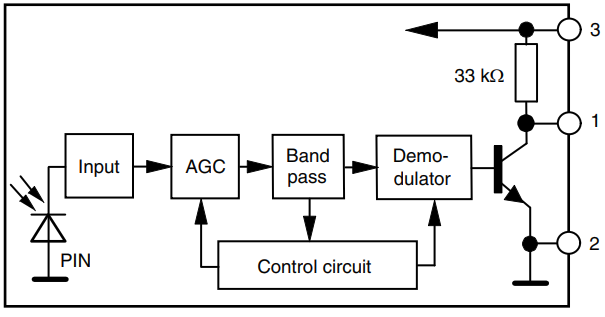
\includegraphics[width=\textwidth]{IR_RX.png}
        \caption{Block diagram of a typical IR receiver module.}
        \label{fig:ir_rx}
    \end{minipage}
\end{figure}

The problem of IR communication is so common that many components (named, unsurprisingly, IR receiver modules) already integrate the circuitry required to capture and demodulate infrared signals, more specifically photodiodes, bandpass filters and demodulators to demodulate the carrier and a pull-up resistor to return an active-low digital signal.\\
Under this premise, the problem of sending IR signals translates to powering an IR LED using a 38KHz carrier while the problem of receiving IR signals translates to sampling values of a digital signal.

\subsubsection{STM32 Nucleo F401RE and the PMDB16 board}
\begin{itemize}
\item The STM32 Nucleo F401RE is a low-power microcontroller board by ST based on an ARM Cortex-M4 CPU core and featuring several I/O ports, I2C / USART / SPI interfaces, timers, a vectored interrupt controller (NVIC) and support for DMA; among all features, its timers can be configured to generate interrupts based on specific events and also generate signals using PWM in capture/compare mode, while its GPIO ports can be configured to generate interrupts on level change.

\item The PMDB16 board was initially designed and manufactured for the Microcontrollers course and later repurposed for the Sensor Systems course at Politecnico di Milano; it is designed to be paired with a ST microcontroller board (or similar, with the same form factor) and features sensors /actuators like photodiodes, potentiometers, LED matrices etc.\\
Among all devices, it also features a IR receiver module (TSOP58238 module) and a IR LED paired with a "class B" amplifier which allows to push more current through the LED than what is usually allowed by the microcontroller pins.
\end{itemize}

\begin{figure}[H]
    \centering
    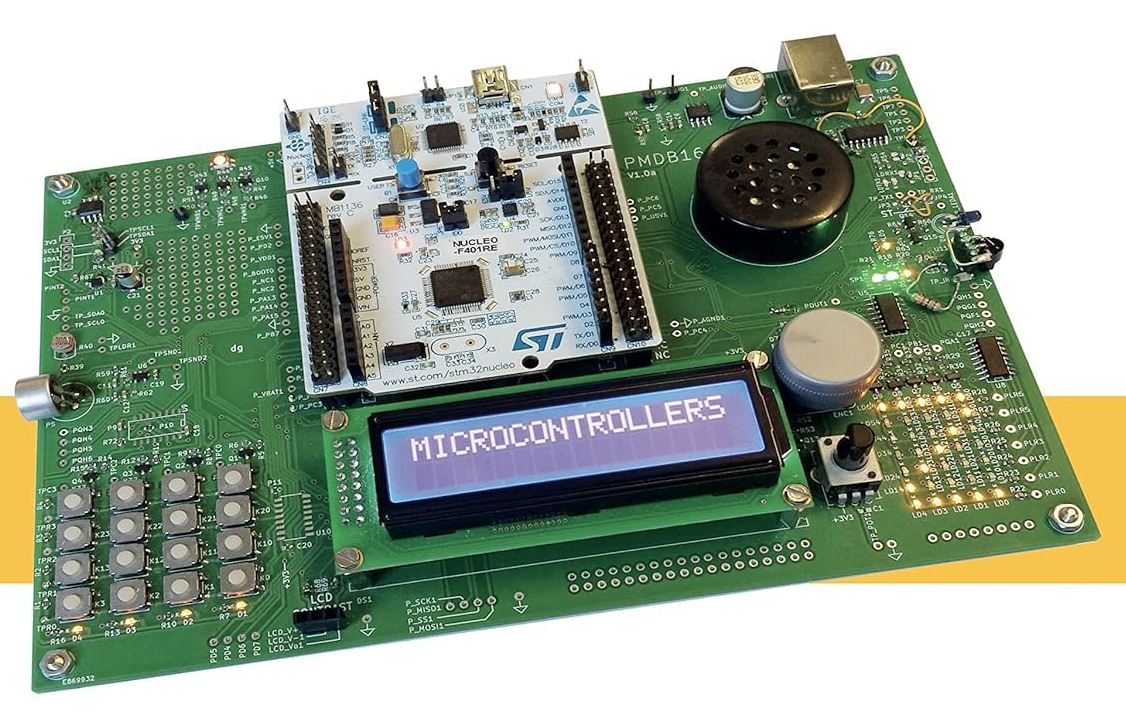
\includegraphics[width=0.5\textwidth]{pmdb16.jpg}
    \caption{The PMD16 board with the STM32F401RE microcontroller board, as it appears on the cover of the book "Microcontrollers" by Franco Zappa.}
    \label{fig:pmdb16}
\end{figure}



\begin{figure}[H]
    \centering
    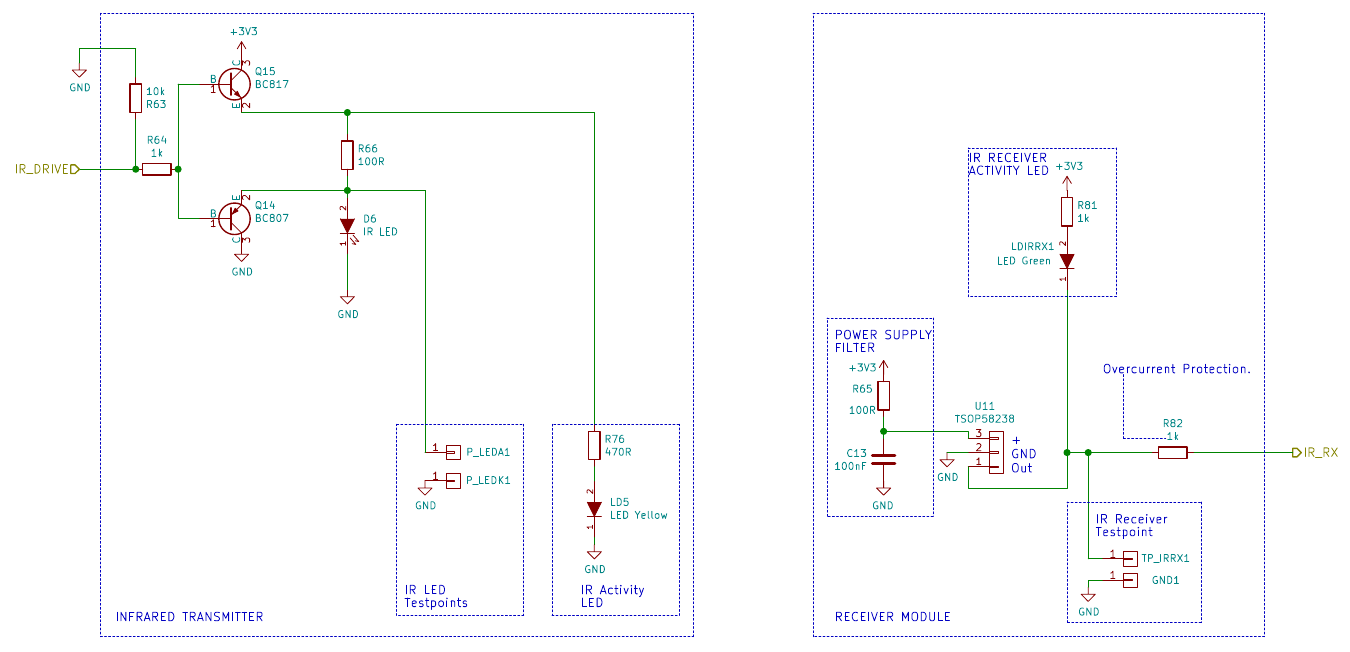
\includegraphics[width=0.8\textwidth]{pmdb16_ir.png}
    \caption{Schematics for the IR receiver and transmitter.}
    \label{fig:pmdb16_ir}
\end{figure}

\subsubsection{Aim of the project}
\textit{This project does not solve any real-world problem that hasn't been (and remained) solved for the last 50 years and is meant to be an opportunity to learn more about microcontroller programming and RTOSes with a hands-on project, thus I'd argue that the aim of the project is the journey itself; indeed, combining concepts prominent in  microcontroller programming like what is essentially memory-mapped I/O with concepts coming from operating systems such as concurrency, scheduling and synchronization mechanisms is a fascinating prospect. The subtle changes in mechanisms and framework w.r.t. plain old microcontroller programming is especially evident when configuring interrupts for devices and using locking mechanisms typical of operating systems.}

\subsection{Design and implementation}
The \texttt{PMDB\_IR} class implements both the sender and the receiver (for a reason that will be clear later), with the \texttt{receive()} function producing a capture and the \texttt{send()} function sending it back.\\
Each capture is a sequence of logic levels and timestamps (in ns).\\
Note: details about register configurations have been left out for brevity, the source code is already well commented.
\subsubsection{IR sender}
In order to send data via the IR LED, the general idea is to connect the IR LED's pin to a timer via alternate function and to generate the carrier in PWM mode, then enable and disable the timer's channel to stimulate the receiver (i.e. send data) at specific timestamps according to the capture.\\
According to ST's user manual, the only timer that can be connected to the IR LED pin \texttt{PB10} via alternate function is \texttt{TIM2 CH3}; for this reason, \text{TIM2} is the timer of choice for the generation of the 38KHz 50\% DC wave.

Implementation:
\begin{itemize}
\item First, \texttt{PB10} (IR LED's pin) is configured in alternate mode with alternate function 1 (\texttt{TIM2 CH3} output) using the API provided by Miosix, while \texttt{TIM2} is configured in capture/compare PWM mode by writing the appropriate registers according to the user manual; notably, \texttt{TIM2} is kept free-running with channel 3 being turned on and off to transmit data. Both configurations happen with IRQs disabled using RAII locks provided by Miosix (\texttt{GlobalIrqLock}) as device registers are subject to concurrency.

\item Inside the \texttt{send()} function, channel 3 of \texttt{TIM2} is turned on and off by writing its bit in the capture/compare register inside a polling loop in order to stimulate the receiver.\\
For each recorded sample, the OS time obtained via \texttt{IRQgetTime()} is compared repeatedly with the timestamp of the current sample; whenever the OS time becomes greater than the timestamp, the channel output is turned on / off accordingly.
\end{itemize}
\subsubsection{IR receiver}
In order to sample the signal coming from the IR receiver, the general idea is to generate interrupts on signal edges coming from the IR receiver's pin and sample the current level and timestamp using a high-resolution timer; the very same timer is also configured to elapse after 1s and generate another interrupt that is then used to stop the sampling.\\
As a rationale for the choices and figures
\begin{itemize}
\item IR signals coming from domestic appliances can range from $\sim500$ baud to 9600 baud and typically feature at most 512 samples (as a pessimistic figure); for this very reason, a recording can last at most $1 / 500 \cdot 512 \approx 1s $ (still, very pessimistic), thus the need to have the recording last at least 1s;\\
\item I decided to stick with a $1\mu s$ timer resolution for the samples, thus requiring to be able to count to at least $1s / 1\mu s = 1000000$ which exceeds the maximum value provided by 16bit timers;\\ according to the ST manual, the only 32bit timers on the microcontroller are \texttt{TIM2} and \texttt{TIM5}, among which the latter is already used as a OS timer (I found this out by trying to register an interrupt for \texttt{TIM5} and seeing Miosix fail over and over in a loop), thus the choice fell again on \texttt{TIM2}; for this very reason, there is a need to be able to reconfigure \texttt{TIM2} based on whether I am sampling or sending IR data since the timer is shared by both functions for different reasons.
\end{itemize}

Implementation:
\begin{itemize}
\item First, \texttt{PA10} (IR receiver's pin) is configured as input using Miosix's API while interrupt generation on signal edge of the pin is configured by routing \texttt{PA10} to \texttt{EXTI10} line,  configuring the \texttt{EXTI RTST / FTSR} registers for interrupts on rising / falling edge and by registering \texttt{isr\_sample()} for the same \texttt{EXTI} line via Miosix's \texttt{IRQregisterIrq()} to sample on each signal edge;\\
\texttt{TIM2}, this time, is configured as a one-pulse 1s timer with a resolution of $1\mu s$ with interrupt generation on timer updates (including when the timer elapses), and \texttt{isr\_stop\_sampling()} is registered for \texttt{TIM2} via \texttt{IRQregisterIrq()} to stop sampling after 1s;
\item Inside the \texttt{receive()} function, both interrupt types are enabled (masked) to start the recording and the function starts sleeping over a condition variable using \texttt{IRQgetCurrentThread()} and \texttt{IRQglobalIrqUnlockAndWait()}; eventually, the condition variable will change and the thread will be woken up with \texttt{cond\_var->IRQwakeup()};
\item \texttt{isr\_sample()}, which is triggered on each signal edge, starts \texttt{TIM2} if it wasn't running already and samples both the value of the pin (low / high) and the current timestamp coming from \texttt{TIM2};
\item \texttt{isr\_stop\_sampling()}, which is triggered when the timer elapses, disables both interrupts and wakes up the sleeping thread to end the recording
\end{itemize}

Notably, since \texttt{TIM2} is shared among two different functions, \texttt{reset\_TIM2()} is used to reset the timer to a default state (and unregister ISRs for good measure) before reconfiguring the timer for sampling (\texttt{configure\_TIM2\_sampler()}) or sending (\texttt{configure\_TIM2\_emitter()}).

\subsubsection{Closing up}
The \texttt{main()} function is written to read the status of the USER button (blue button on the Nucleo board) and either sample or send data via IR with a short press of the button or toggle between the two modes with a long press ($\geq 1s$); it also prints a cool TUI over serial to show the current state of the application, even though the application also works "headless". Although of interest, how it was implemented is out of the scope of the project.

\section{Project outcomes}

\subsection{Concrete outcomes}

Produced artifacts:
\begin{itemize}
\item \texttt{main.cpp} containing the logic to start recording / sending IR data, toggling between modes and printing status
\item \texttt{PMDB\_IR.hpp} containing the \texttt{PMDB\_IR} class implementing the sampling and receiving logic
\item Waveform dumps in VCD format, either produced by using a logic analyzer during the early stages of the project or synthesized by the \texttt{receive()} function for debugging / verification purposes
\item A Python script to convert a VCD file into the internal representation used by my program for debugging purposes
\item This report
\end{itemize}

\subsection{Learning outcomes}

My most important outcomes are:
\begin{itemize}
\item I improved in navigating other people's codebases, more specifically Miosix's, which enabled me to have a deeper understanding of the API functions that I was using and to look at usage examples
\item I improved in reading technical documentation, more specifically the Nucleo manual; now long technical documents are less scary
\item I learned how microcontroller devices are configured at the low level as opposed to using a high-level API (e.g. STM HAL)
\item I learned and reasoned about how digital signals are sampled, what tools I have under my belt in order to do so (e.g. polling vs interrupts); I will probably use this knowledge to build my own logic analyzer for fun (and profit, auspicably)
\item I had a deeper look at how operating systems are structured and how they accommodate available devices on the microcontroller / platform
\item I learned how to use a logic analyzer
\end{itemize}

I still have doubts about synchronisation primitives, my experience was mostly focused on device configuration.

\subsection{Existing knowledge}
Previous knowledge that has aided in finishing this project:
\begin{itemize}
\item Attending the Sensor Systems course introduced me to embedded systems programming, although at a higher abstraction level, to the point that I expected the Embedded Systems course to trace the same steps at a lower level, and it seriously helped in doing this project
\item Attending the Digital Electronic Systems Design course also helped to some extent in terms of understanding how microcontroller devices work and how they are implemented at the RTL level
\end{itemize}

\subsection{Problems encountered}
The biggest problems that I encountered are:
\begin{itemize}
\item Finding out that I was constrained to using \texttt{TIM2} only for different purposes and that I had to find a way to reconfigure it in between uses
\item I found myself being out of reach of a logic analyzer for 2 entire days, thus being unable to formally verify behaviour and to debug problems
\end{itemize}

\section{Honor Pledge}

I pledge that this work was fully and wholly completed within the criteria
established for academic integrity by Politecnico di Milano (Code of Ethics and
Conduct) and represents my original production, unless otherwise cited.

I also understand that this project, if successfully graded,  will fulfill part B requirement of the
Advanced Operating System course and that it will be considered valid up until
the AOS exam of Sept. 2026.

\begin{flushright}
\includegraphics[]{firma.png}
\end{flushright}

\end{document}
